\documentclass{article} 
  \author{Name:JIE CAO \quad ID:27510964 \quad Email:jc3g15@soton.ac.uk} 
  \title{Machine Learning Assignment} 
  \usepackage{amsmath} 
  \usepackage{amssymb}
  \usepackage{graphicx}
  \usepackage{float}
  \usepackage{color}
  \usepackage{subfigure}
  \usepackage{geometry}
  \geometry{left=2cm,right=2cm,top=0.1cm,bottom=2cm}
\begin{document} 
\maketitle 
\section{Bayes optimal boundary \& Neural Network Approximation}
\begin{figure}[htbp]
 \centering
 \subfigure[Decision boundary]
 {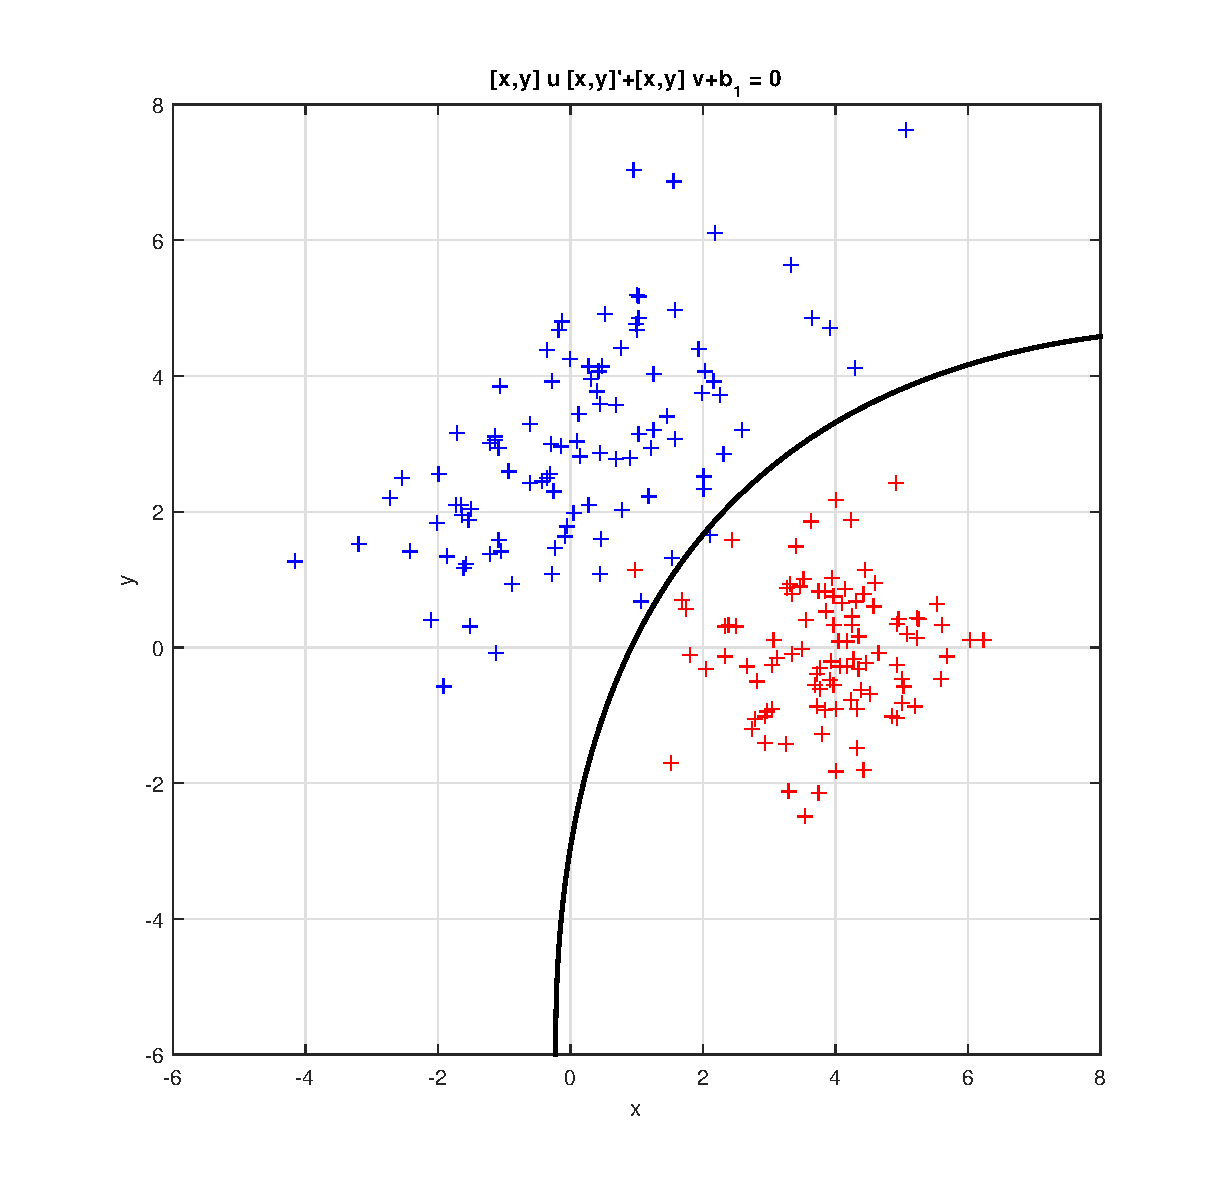
\includegraphics[width=0.43\textwidth]{image/1.eps}}
 \subfigure[Three dimensional graph]
 {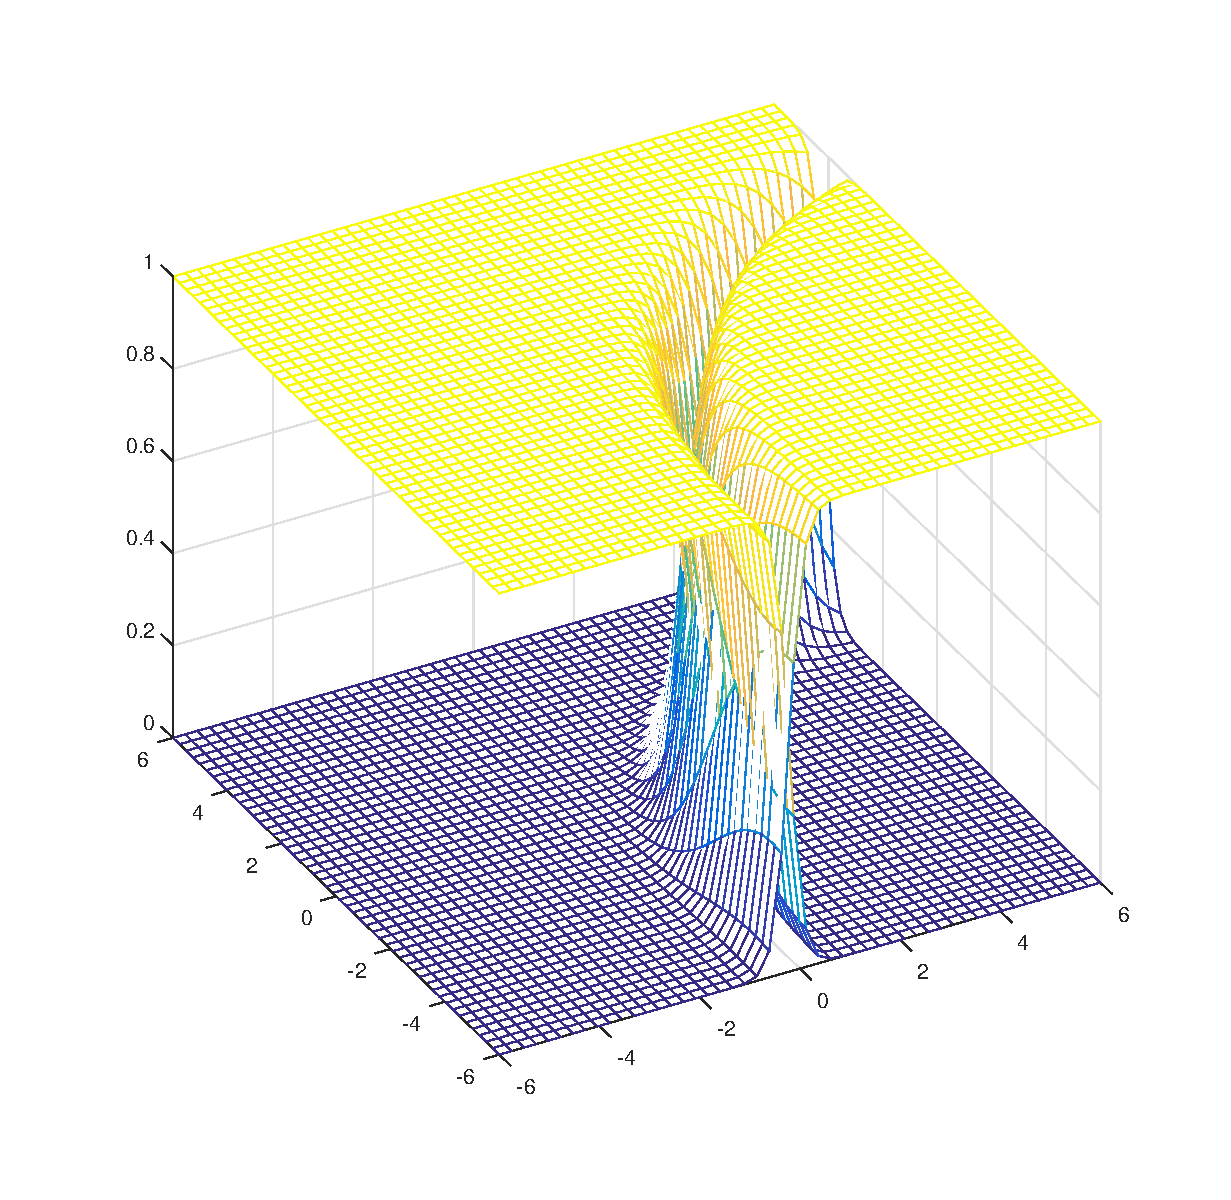
\includegraphics[width=0.43\textwidth]{image/2.eps}}
 \caption{Bayes' optimal boundary}
\end{figure}
\paragraph{•}
\begin{figure}[htbp]
 \centering
 \subfigure[20 hidden nodes]
 {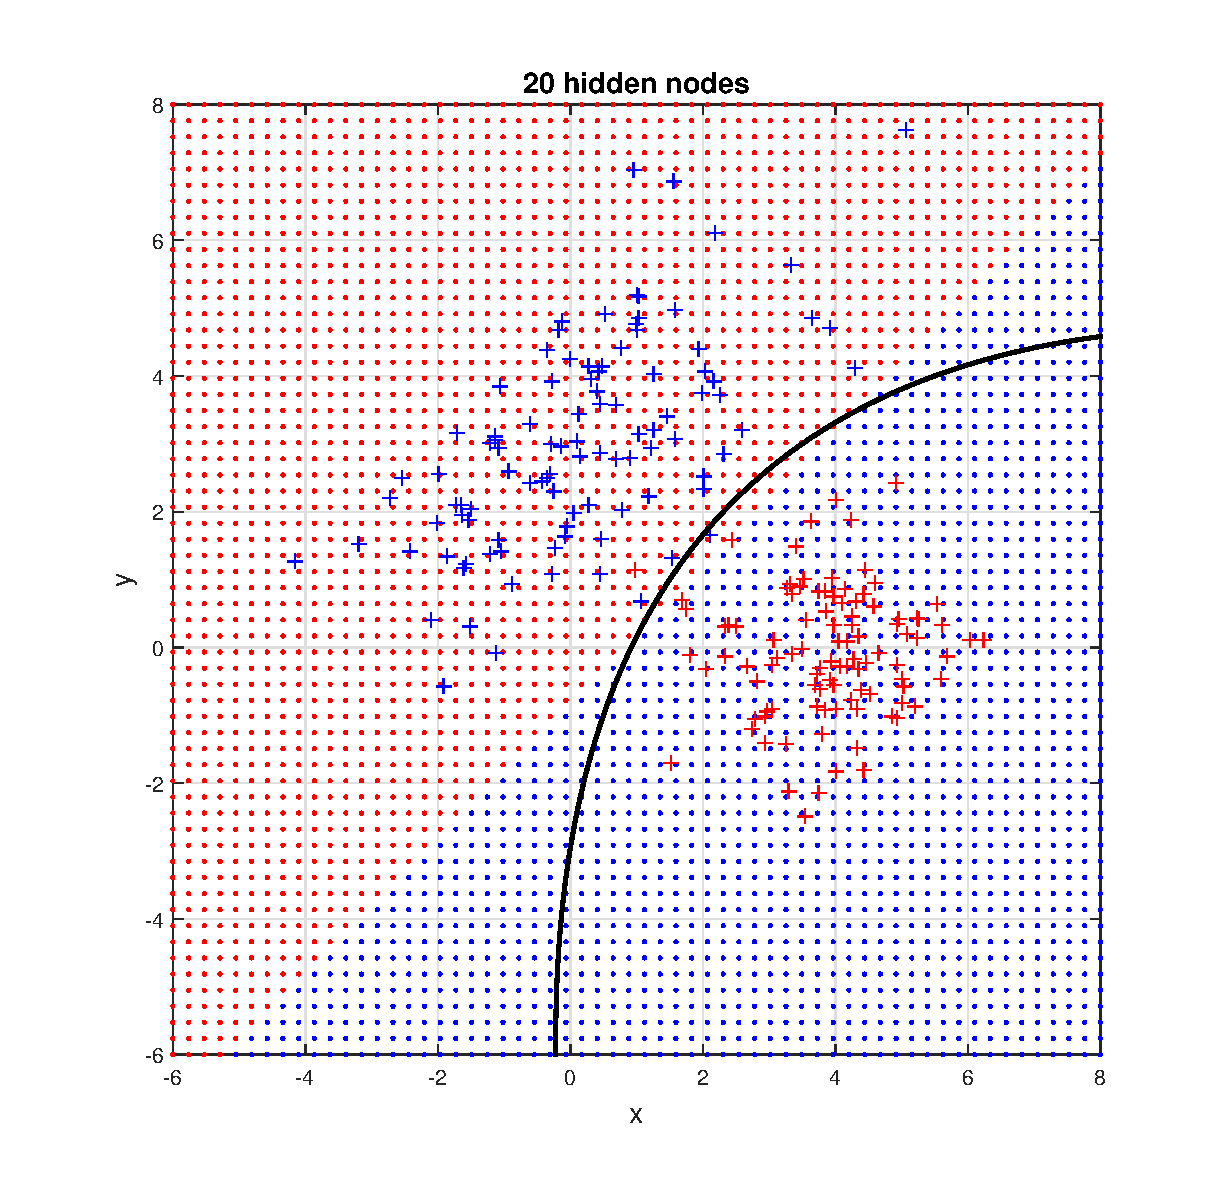
\includegraphics[width=0.32\textwidth]{image/3.eps}}
 \subfigure[30 hidden nodes]
 {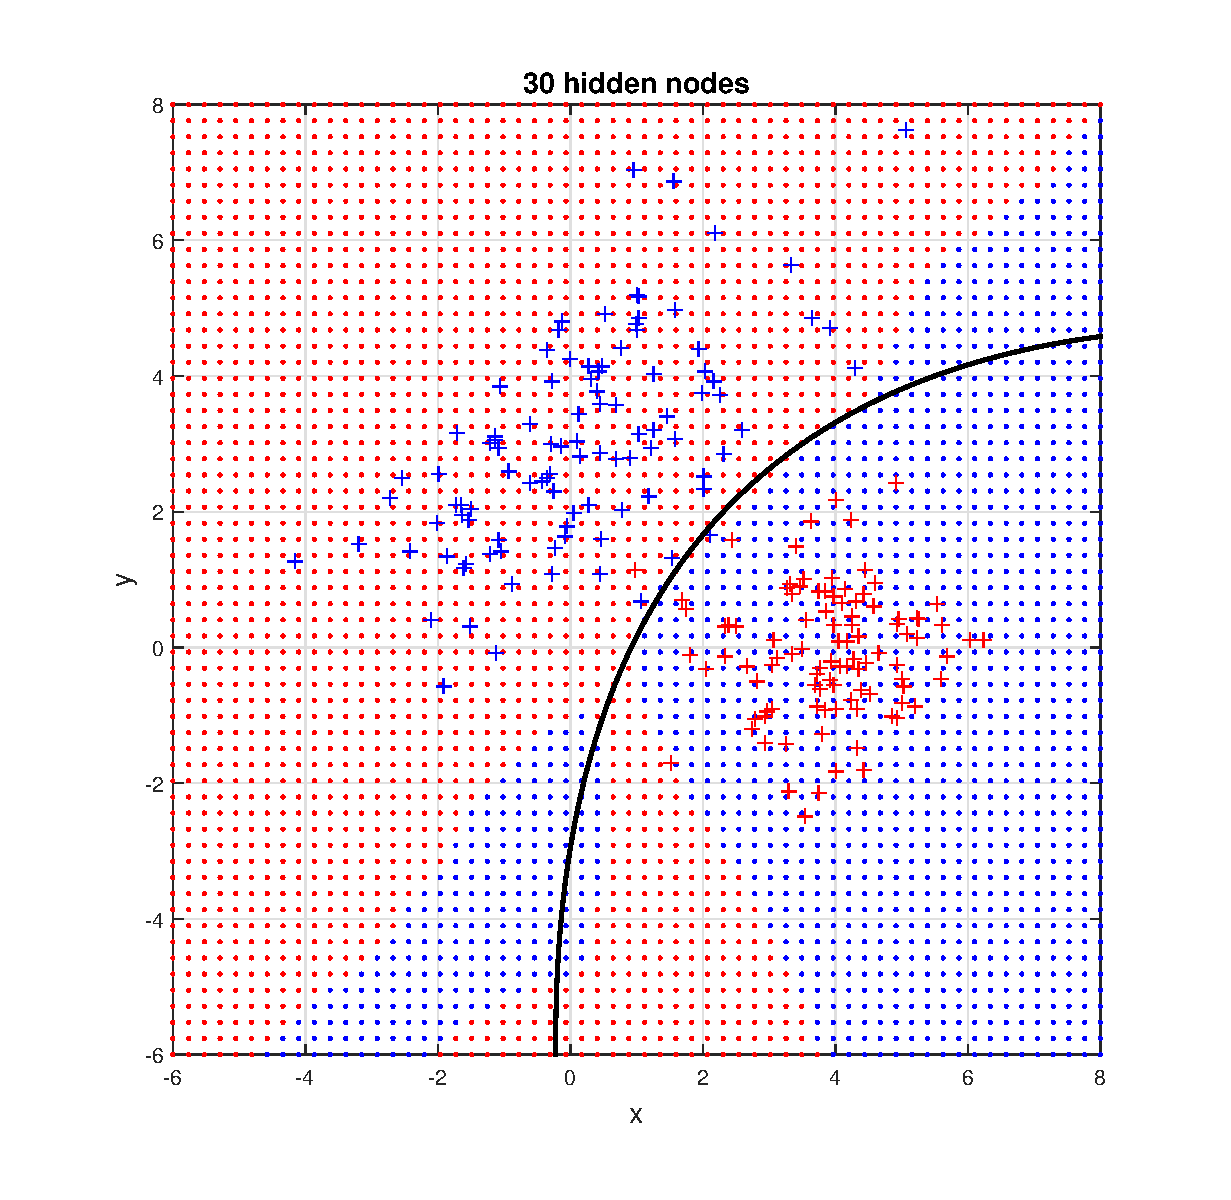
\includegraphics[width=0.32\textwidth]{image/3A2.eps}}
 \subfigure[100 hidden nodes]
 {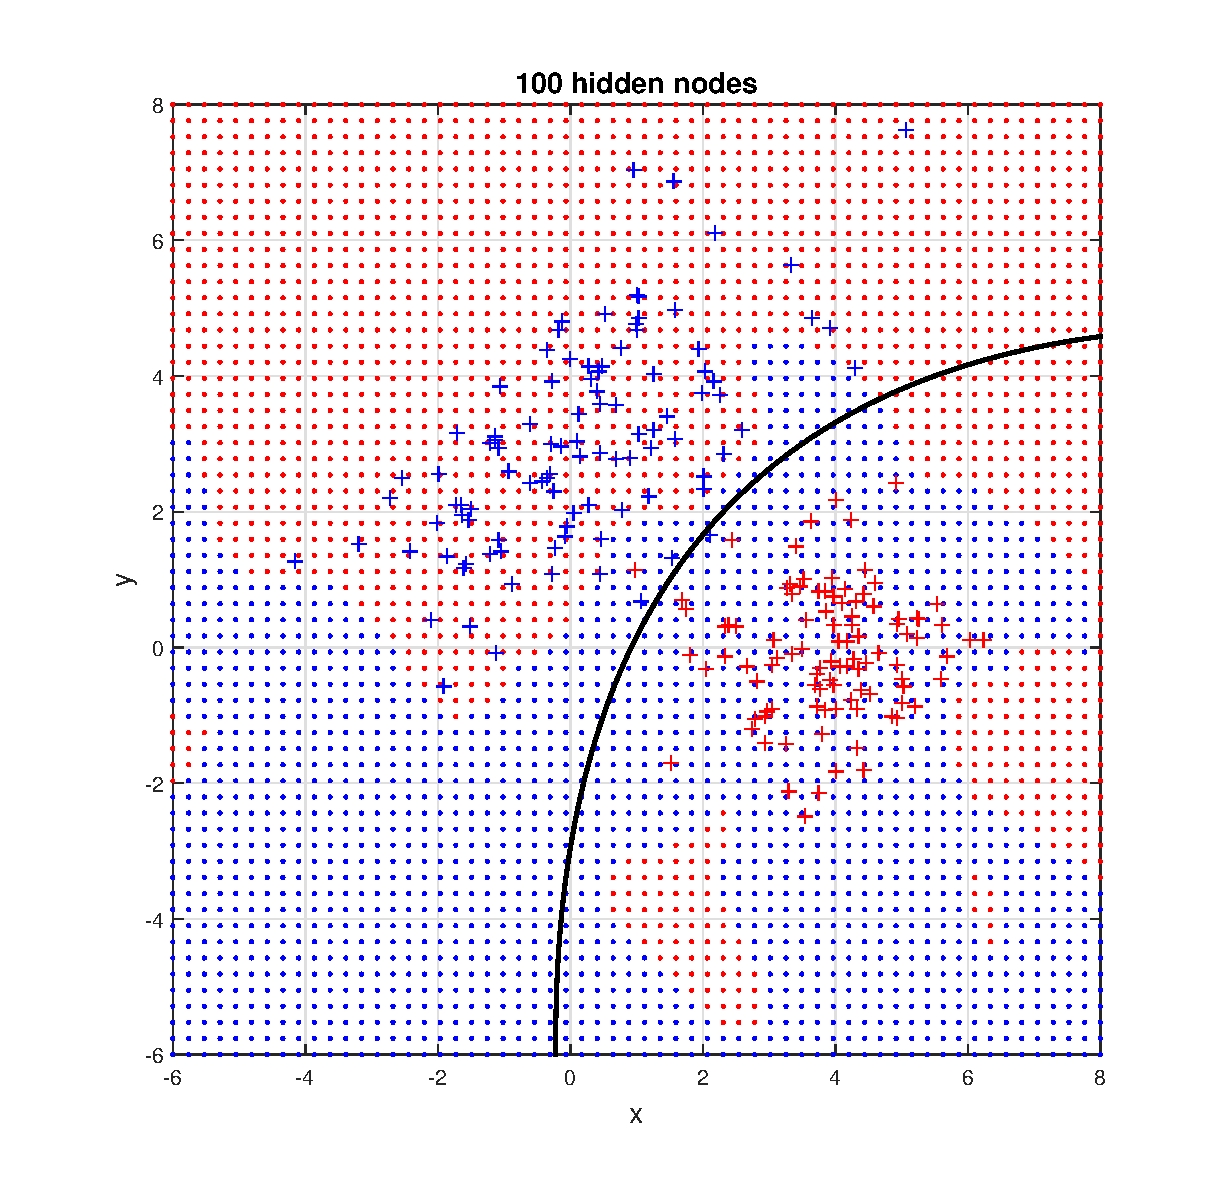
\includegraphics[width=0.32\textwidth]{image/3A3.eps}}
 \caption{Neural network}
\end{figure}
\paragraph{•}The more the hidden nodes are, the better the neural network fit training data. Bayes' optimal boundary's accuracy is better than neural network's.
\newpage 
\section{Time Series Prediction}
\paragraph{•}The Mackey-Glass model is a popular chaotic time series. It is obtained by integrating the non-linear differential equation:
\[
	\left. 
      \dfrac{dx}{dt}=
    \right.
    \left. 
      \dfrac{ax(t-\tau)}{1+x(t-\tau)^{10}}-bx(t)
    \right.
\]
\paragraph{•}The figure of time series:
\begin{figure}[htbp]
 \centering
 \subfigure[generate 2000 samples]
 {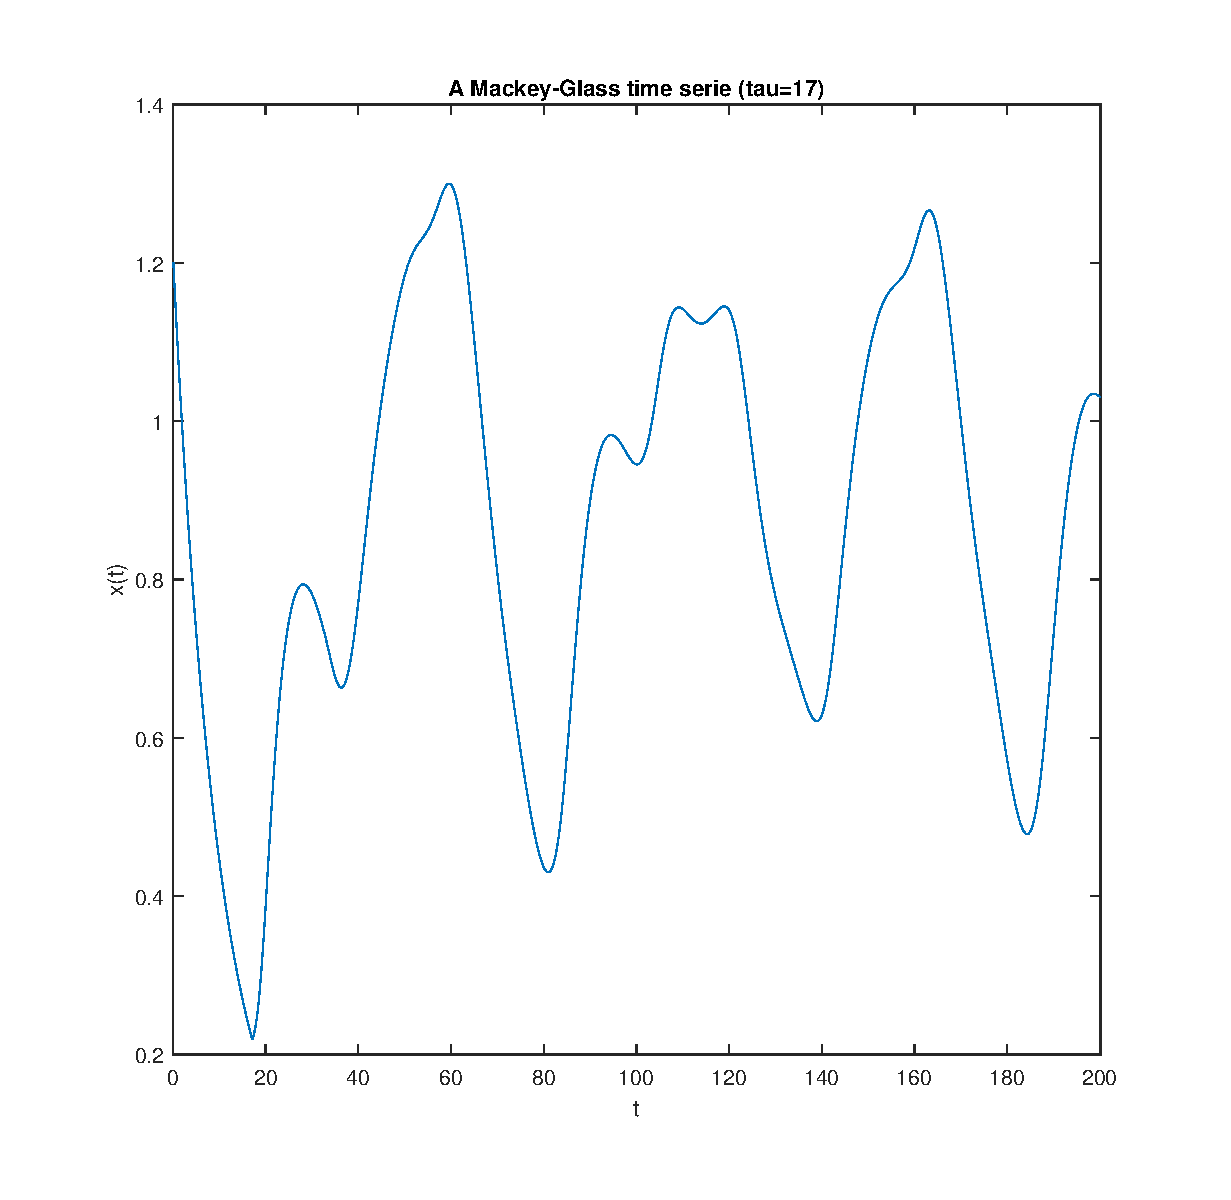
\includegraphics[width=0.58\textwidth]{image/10.eps}}
 \caption{chaotic time series}
\end{figure}
\paragraph{•}One step predicted value was almost same as the true value. when I used free running mode to predict value, the outcome was good at the beginning. but the predicted value would be very inaccurate later. Because the predicted output is dependent on previous 20 values. In free running model, these previous 20 values will be replaced by predicted values with the processing of prediction(feed back predicted outputs into the input). That means these previous 20 values will be more and more unauthentic. Using neural network to do free running model resulted sustained oscillations.
	$$(p=20,\quad N_{tr}=1500,\quad N=2000)$$
\bigskip 
 \[
 	\left. 
      Training\quad
    \right. 
	\left[ 
    \begin{array}{ccccc} 
    	1 & 2 & \cdots & 19 & 1 \\ 
        2 & 3 & \cdots & 20 & 1 \\
        \vdots & \vdots &\quad& \vdots & \vdots \\
        N_{tr}-p+1 & N_{tr}-p+2 & \cdots & N_{tr}-1 & 1 
    \end{array} 
    \right]
    \left[ 
    \begin{array}{c} 
    	w_{1} \\ 
        w_{2} \\
        \vdots \\
        w_{20} 
    \end{array} 
    \right]
    \left. 
      =
    \right. 
    \left[ 
    \begin{array}{c} 
    	p \\ 
        p+1 \\
        \vdots \\
        N_{tr} 
    \end{array} 
    \right]
 \]
 \bigskip 
 \[
 	\left. 
      Test\quad
    \right. 
	\left[ 
    \begin{array}{ccccc} 
    	N_{tr}-p+2 & N_{tr}-p+3 & \cdots & N_{tr} & 1 \\ 
        N_{tr}-p+3 & N_{tr}-p+4 & \cdots & N_{tr}+1 & 1 \\ 
        \vdots & \vdots &\quad& \vdots & \vdots \\
        N-p+1 & N-p+2 & \cdots & N-1 & 1 
    \end{array} 
    \right]
    \left[ 
    \begin{array}{c} 
    	w_{1} \\ 
        w_{2} \\
        \vdots \\
        w_{20} 
    \end{array} 
    \right]
    \left. 
      =
    \right. 
    \left[ 
    \begin{array}{c} 
    	N_{tr}+1 \\ 
        N_{tr}+2 \\
        \vdots \\
        N 
    \end{array} 
    \right]
 \]
\begin{figure}[htbp]
 \centering
 \subfigure[Linear predictor]
 {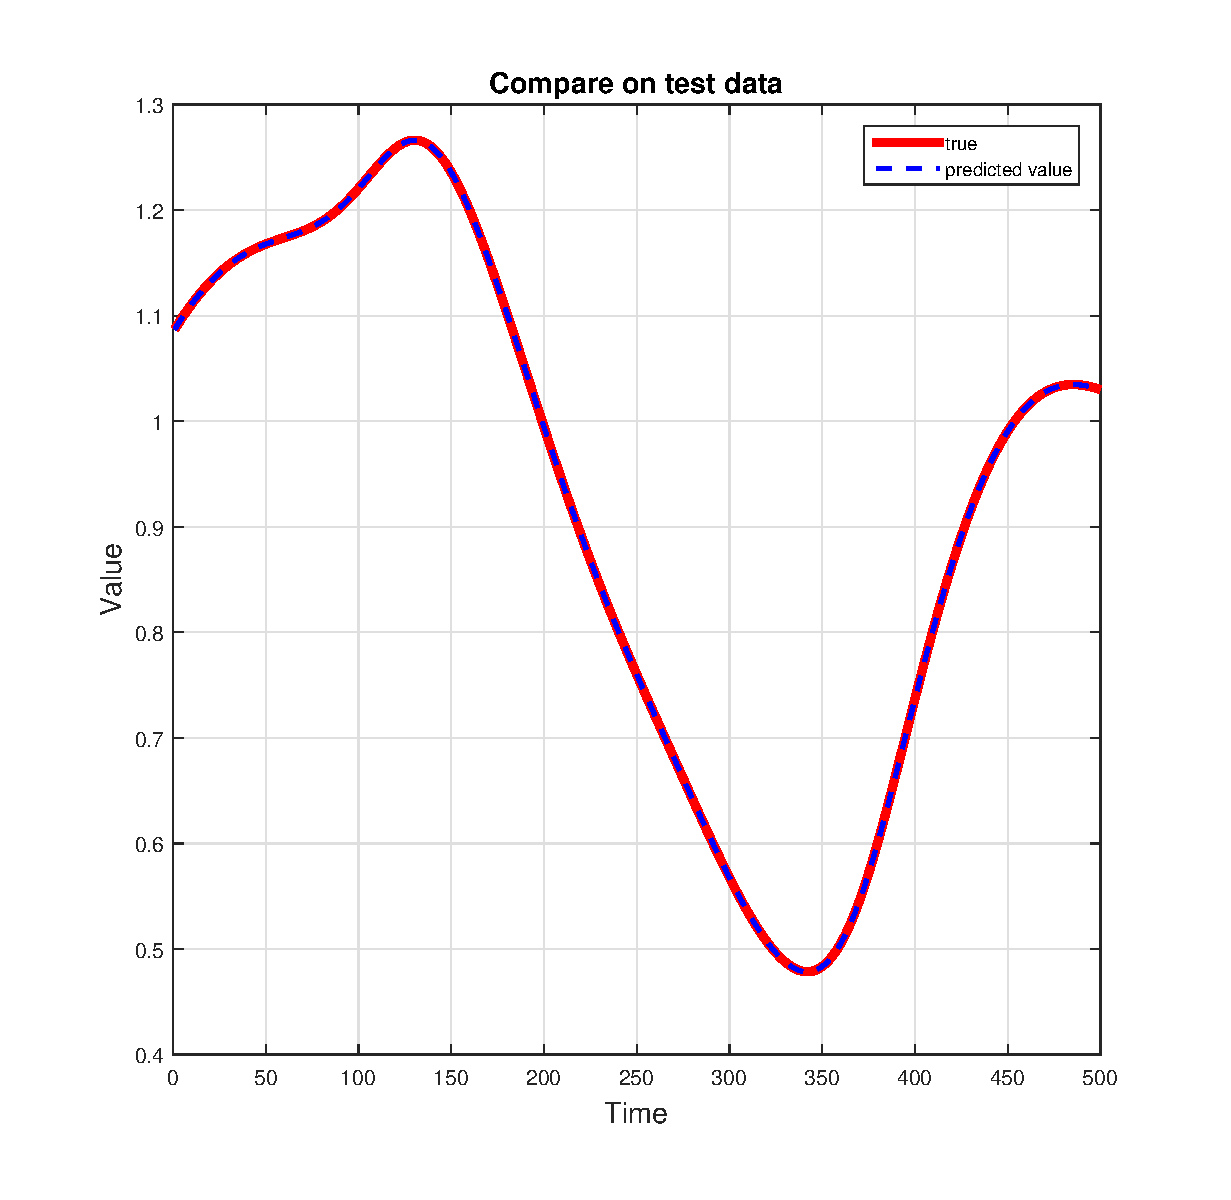
\includegraphics[width=0.43\textwidth]{image/4.eps}}
 \subfigure[Feedforward neural network]
 {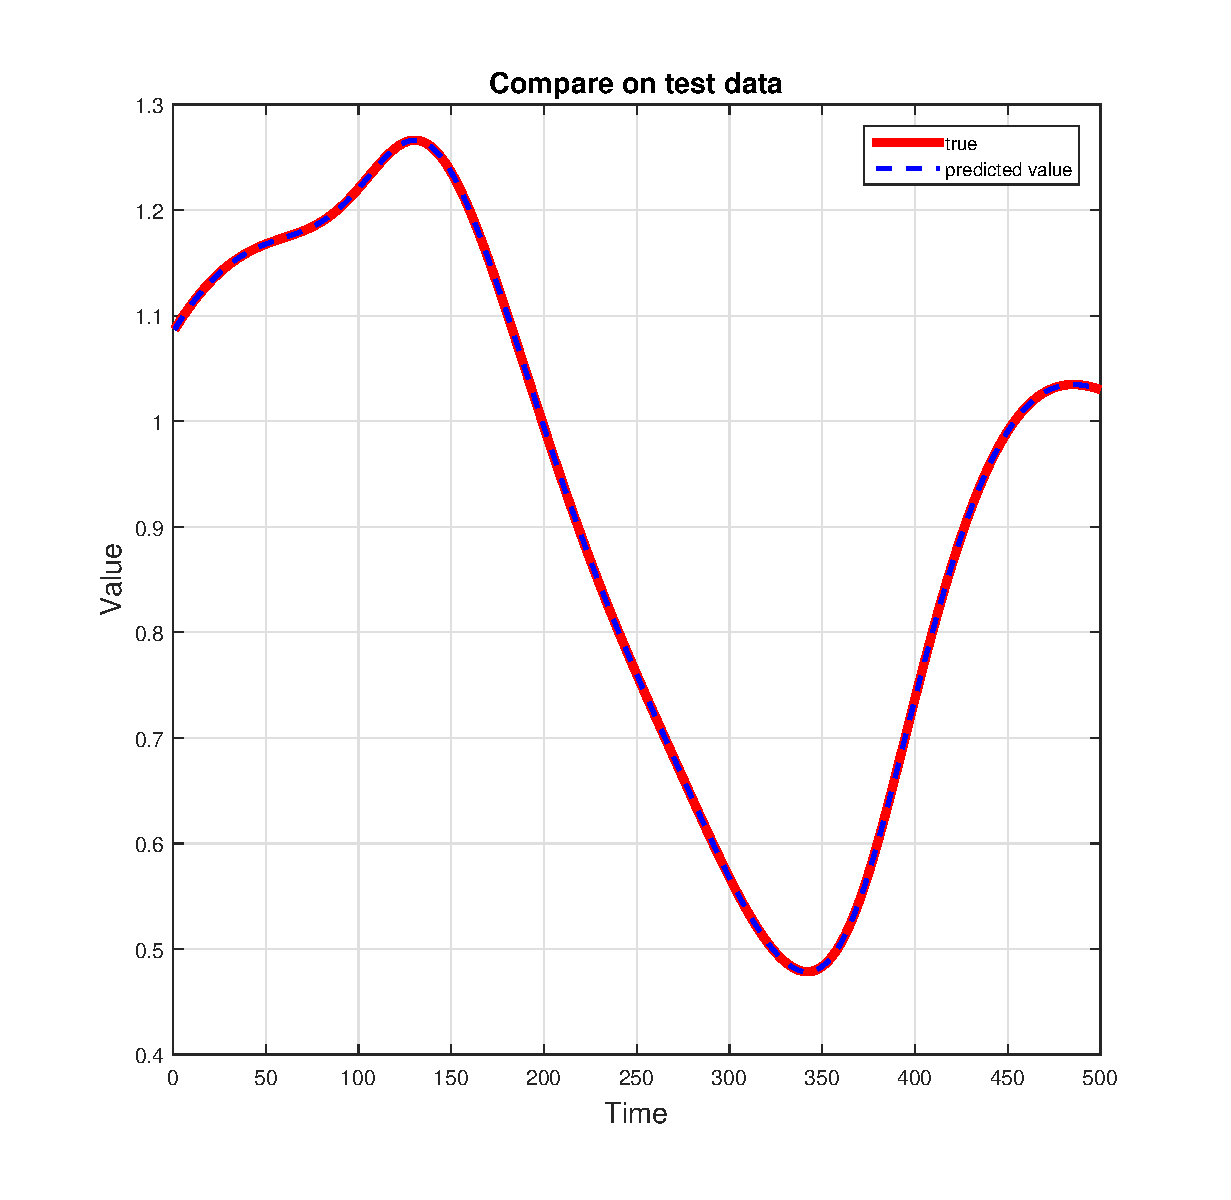
\includegraphics[width=0.43\textwidth]{image/5.eps}}
 \caption{One step ahead prediction}
\end{figure}
\newpage 
\begin{figure}[htbp]
 \centering
 \subfigure[Linear predictor]
 {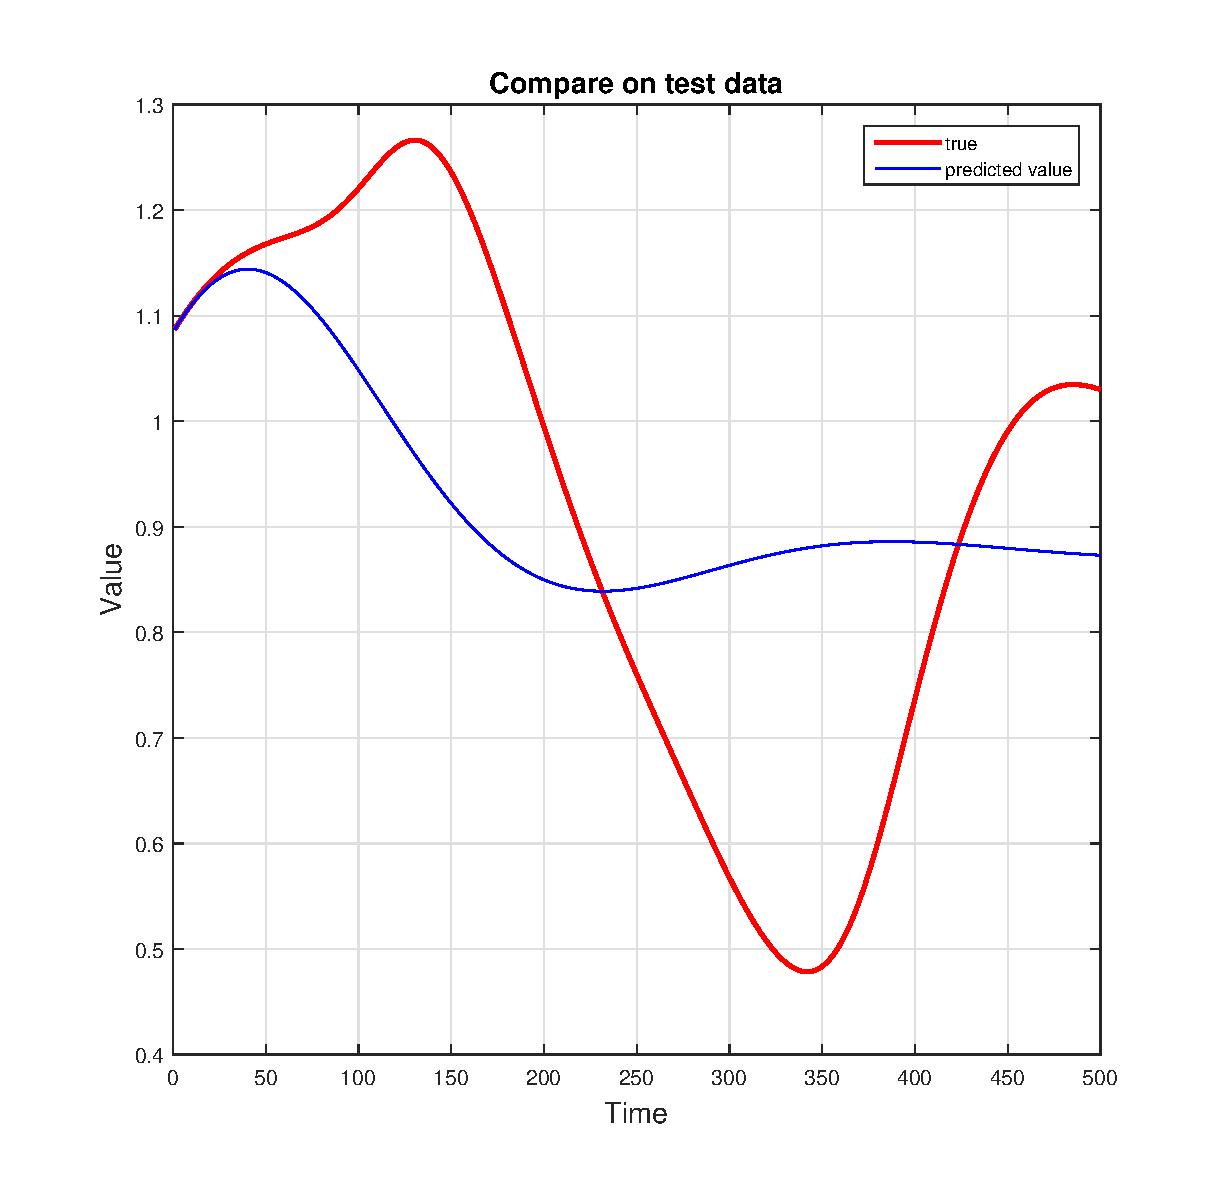
\includegraphics[width=0.43\textwidth]{image/6.eps}}
 \subfigure[Feedforward neural network]
 {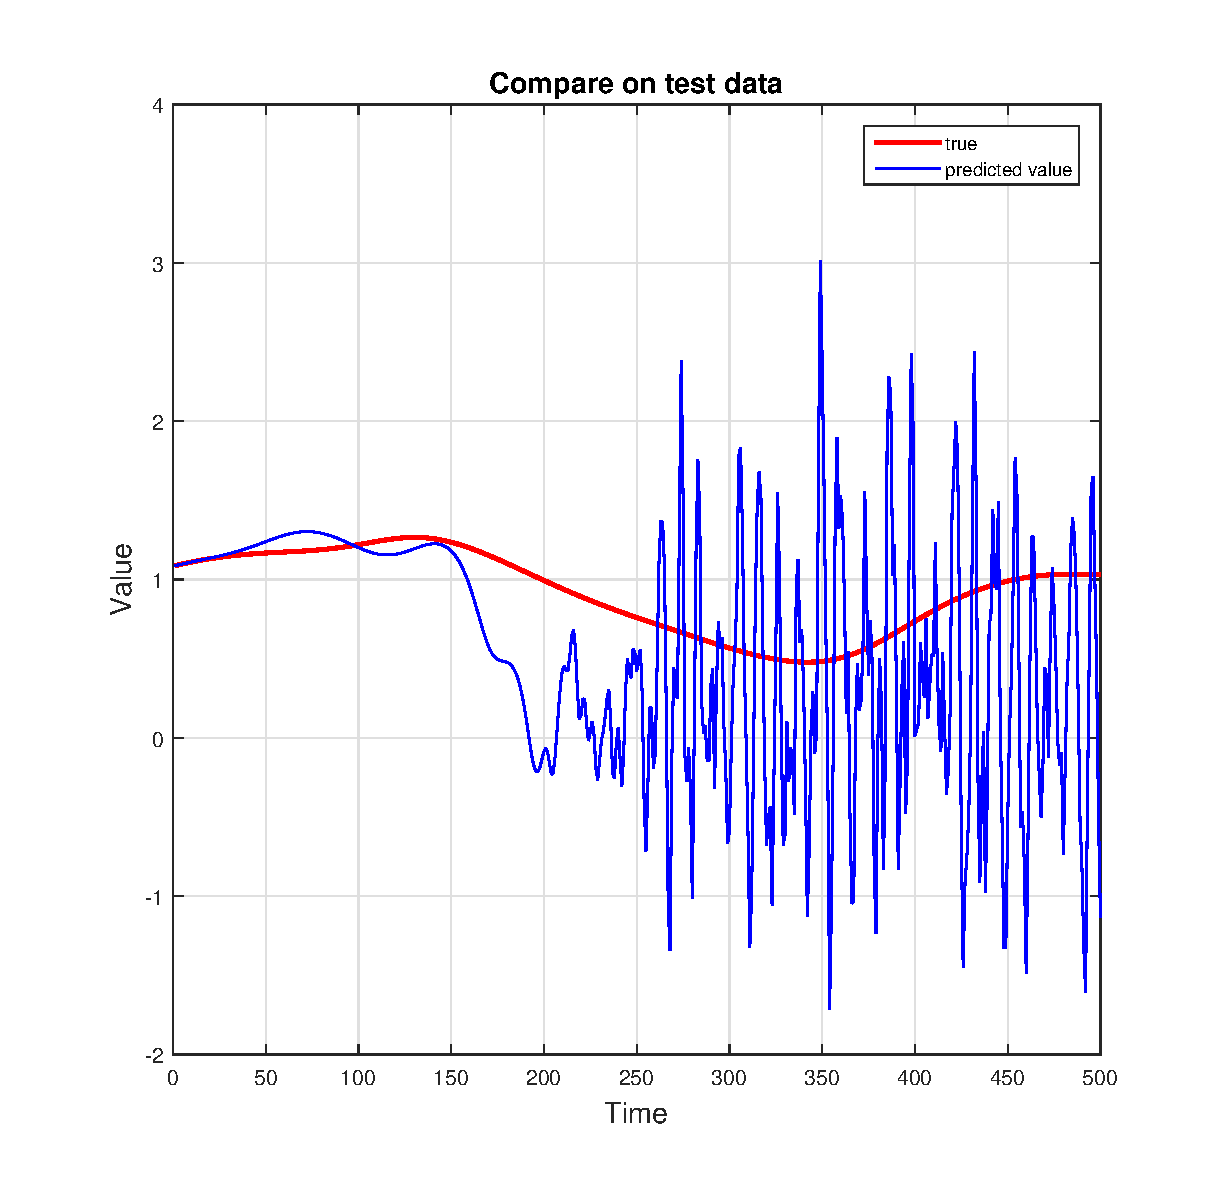
\includegraphics[width=0.43\textwidth]{image/7.eps}}
 \caption{Free running model}
\end{figure}
\section{Financial Time Series}
\paragraph{•}I've download the finance data from 2011/1/3 to 2015/11/27 to train and validate. The last 10 days are used to validate.
\paragraph{•}I used multi-step ahead prediction to predict the close prices in next 10 days. 1-10 step ahead prediction is like one step ahead prediction. In one step, we use data from day 1 to 19 to predict the close price of day 20. In two step, we use data from 1 to 19 to predict the close price of day 21. Doing this 10 times can get 10 close prices in next 10 days. The difference between different step prediction is just the time interval. 1 step predicts next day's price. 2 step predicts the price of the day after tomorrow. 
\newpage 
\begin{figure}[htbp]
 \centering
 \subfigure[Close prices of 10 days before 2015/11/27]
 {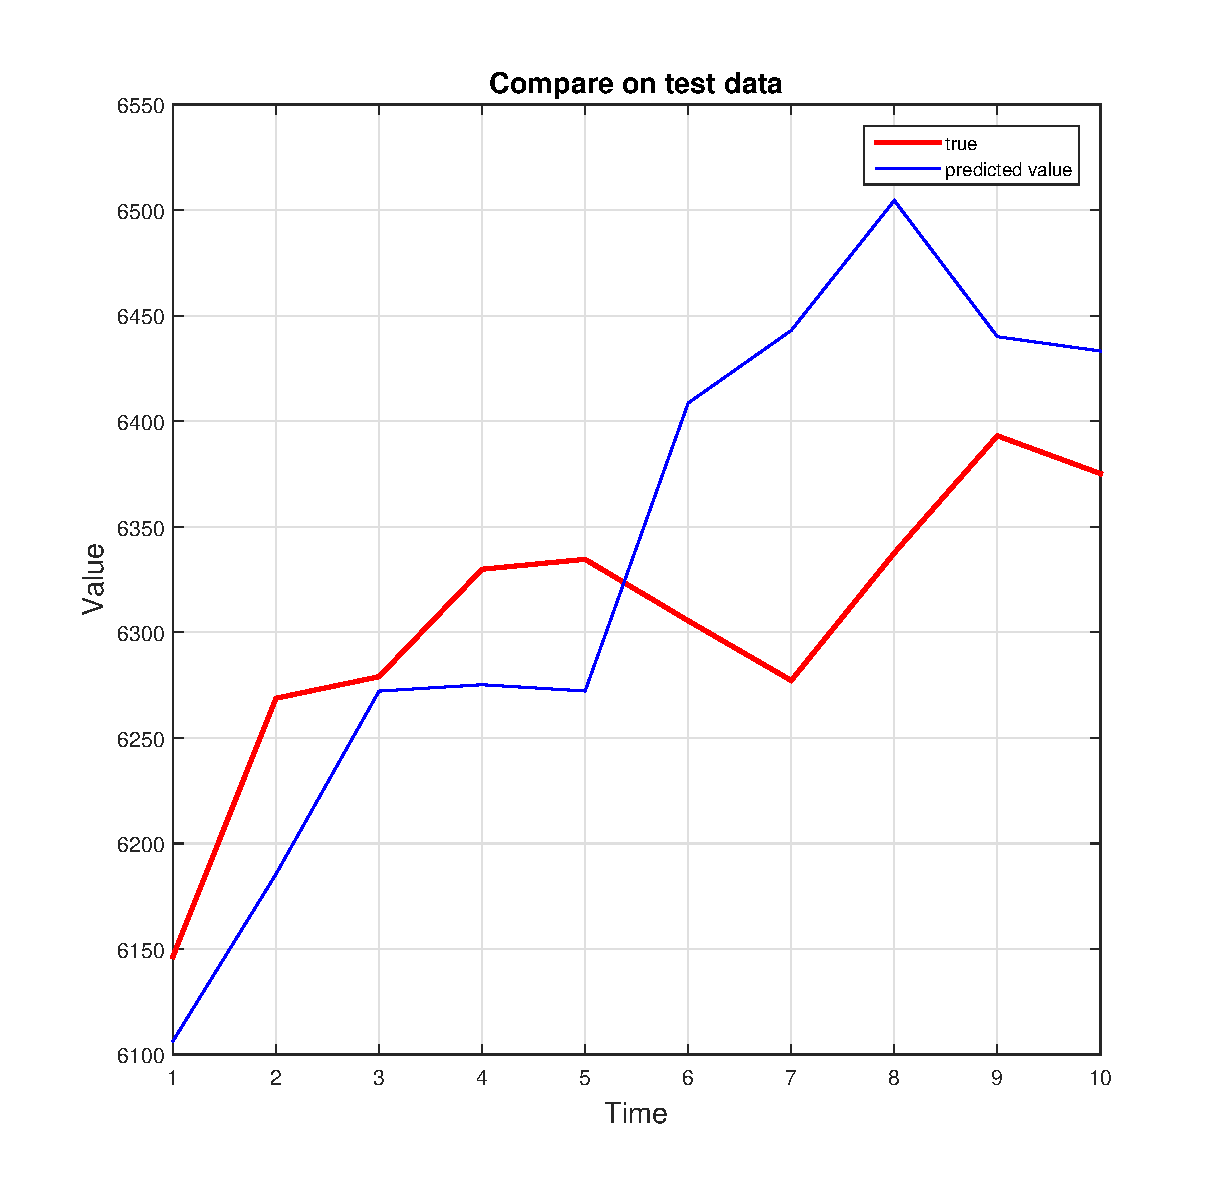
\includegraphics[width=0.45\textwidth]{image/9.eps}}
 \subfigure[Predicted output values]
 {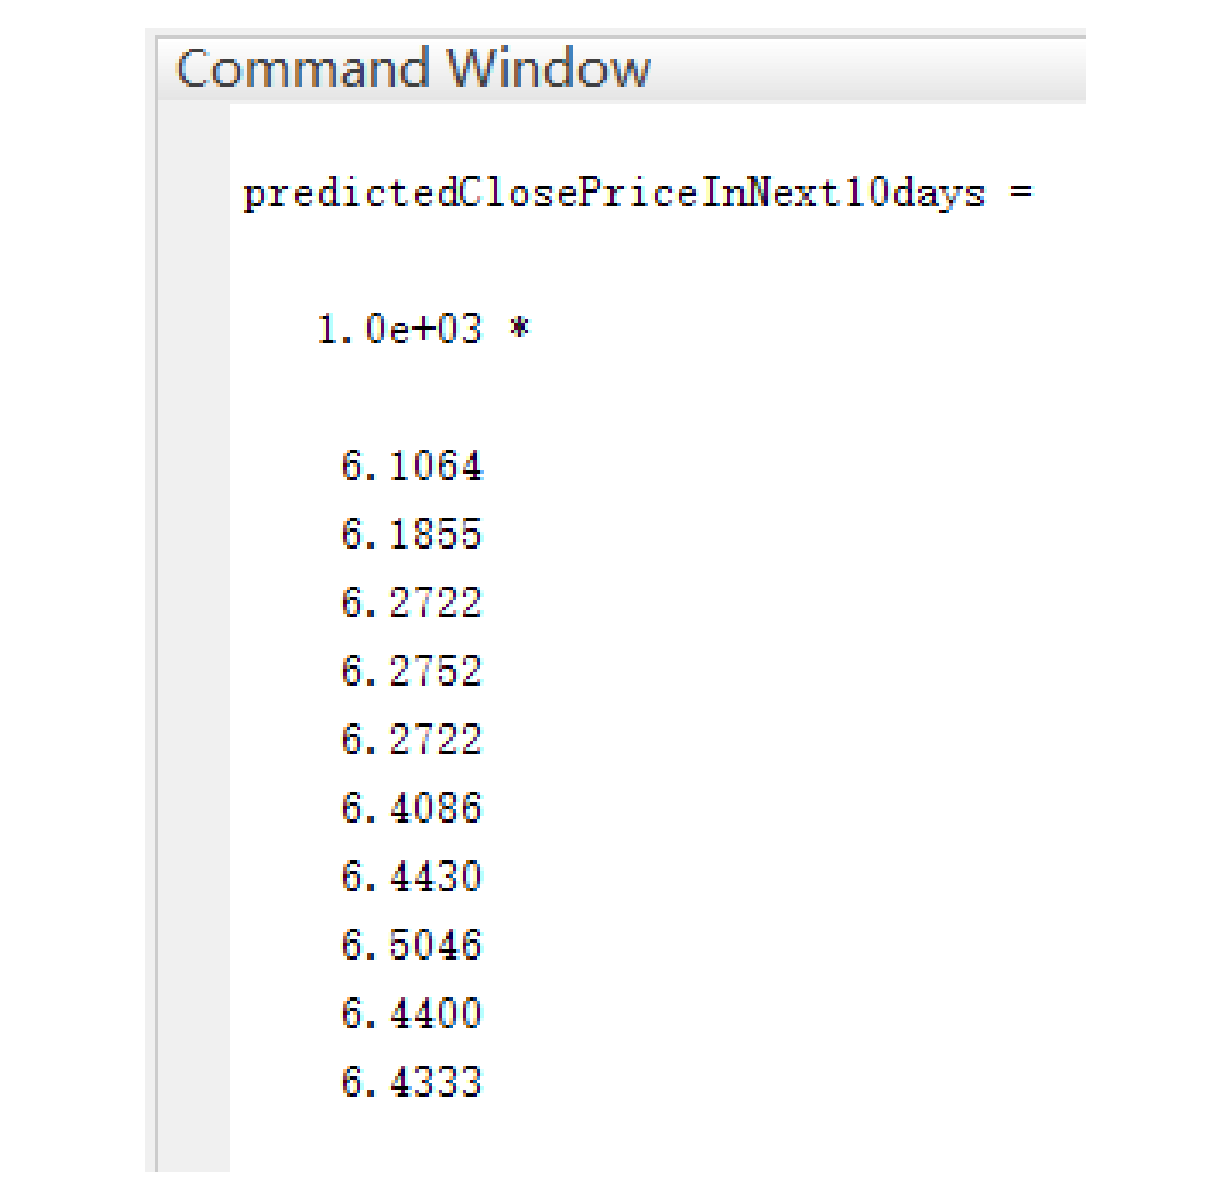
\includegraphics[width=0.45\textwidth]{image/9command.eps}}
 \caption{1-10 step ahead prediction}
\end{figure}
\begin{figure}[htbp]
 \centering
 \subfigure[Close prices of 10 days before 2015/11/27]
 {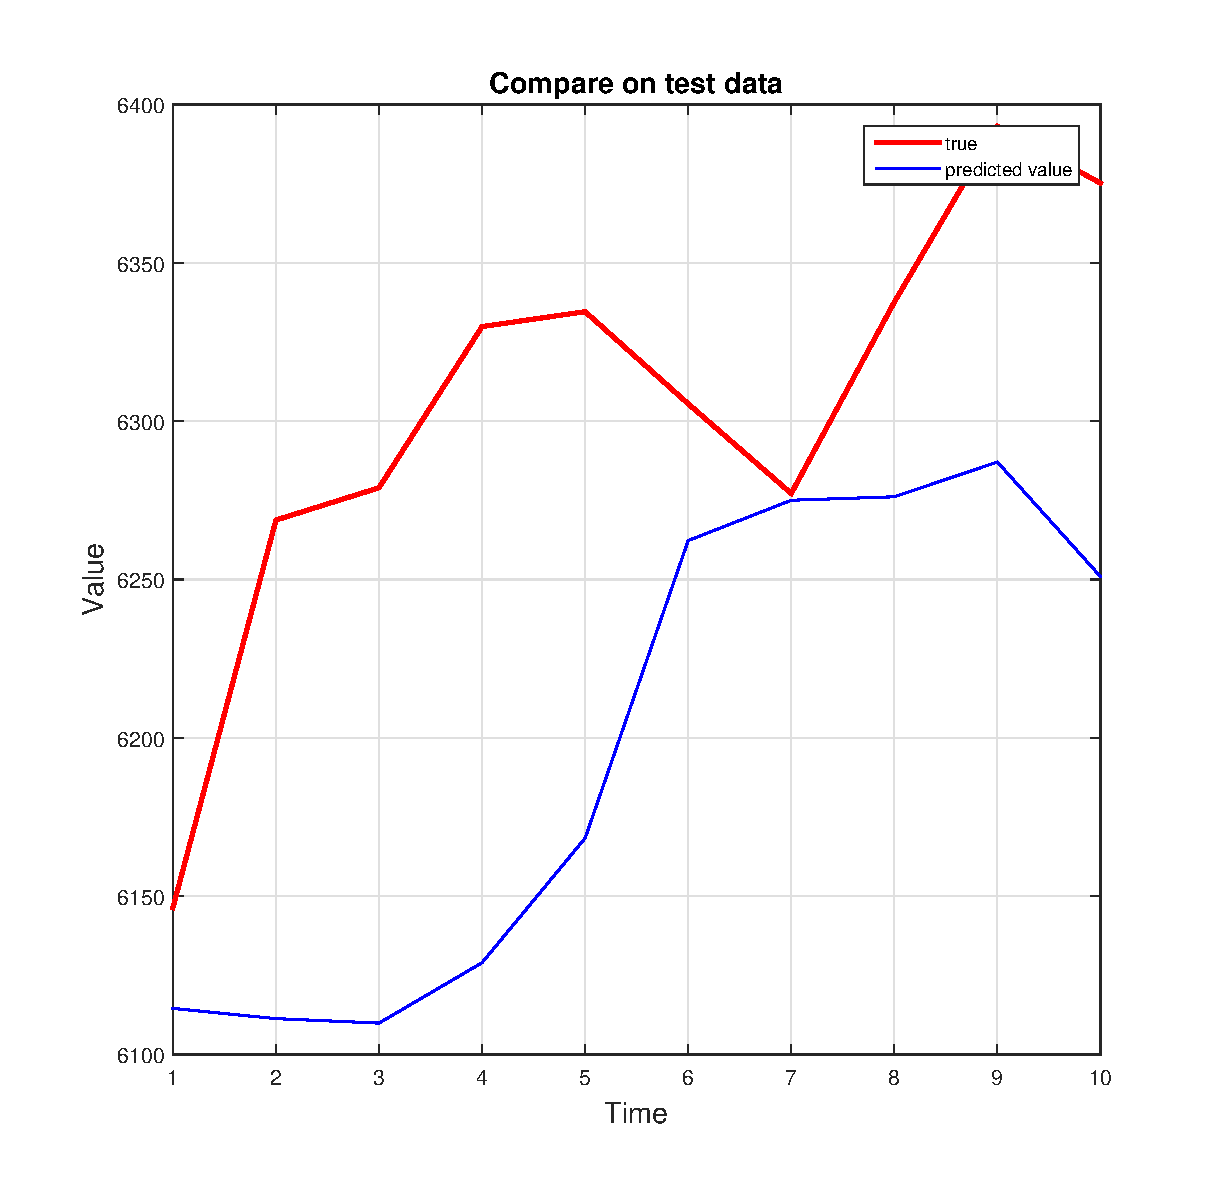
\includegraphics[width=0.45\textwidth]{image/8.eps}}
 \subfigure[Predicted output values]
 {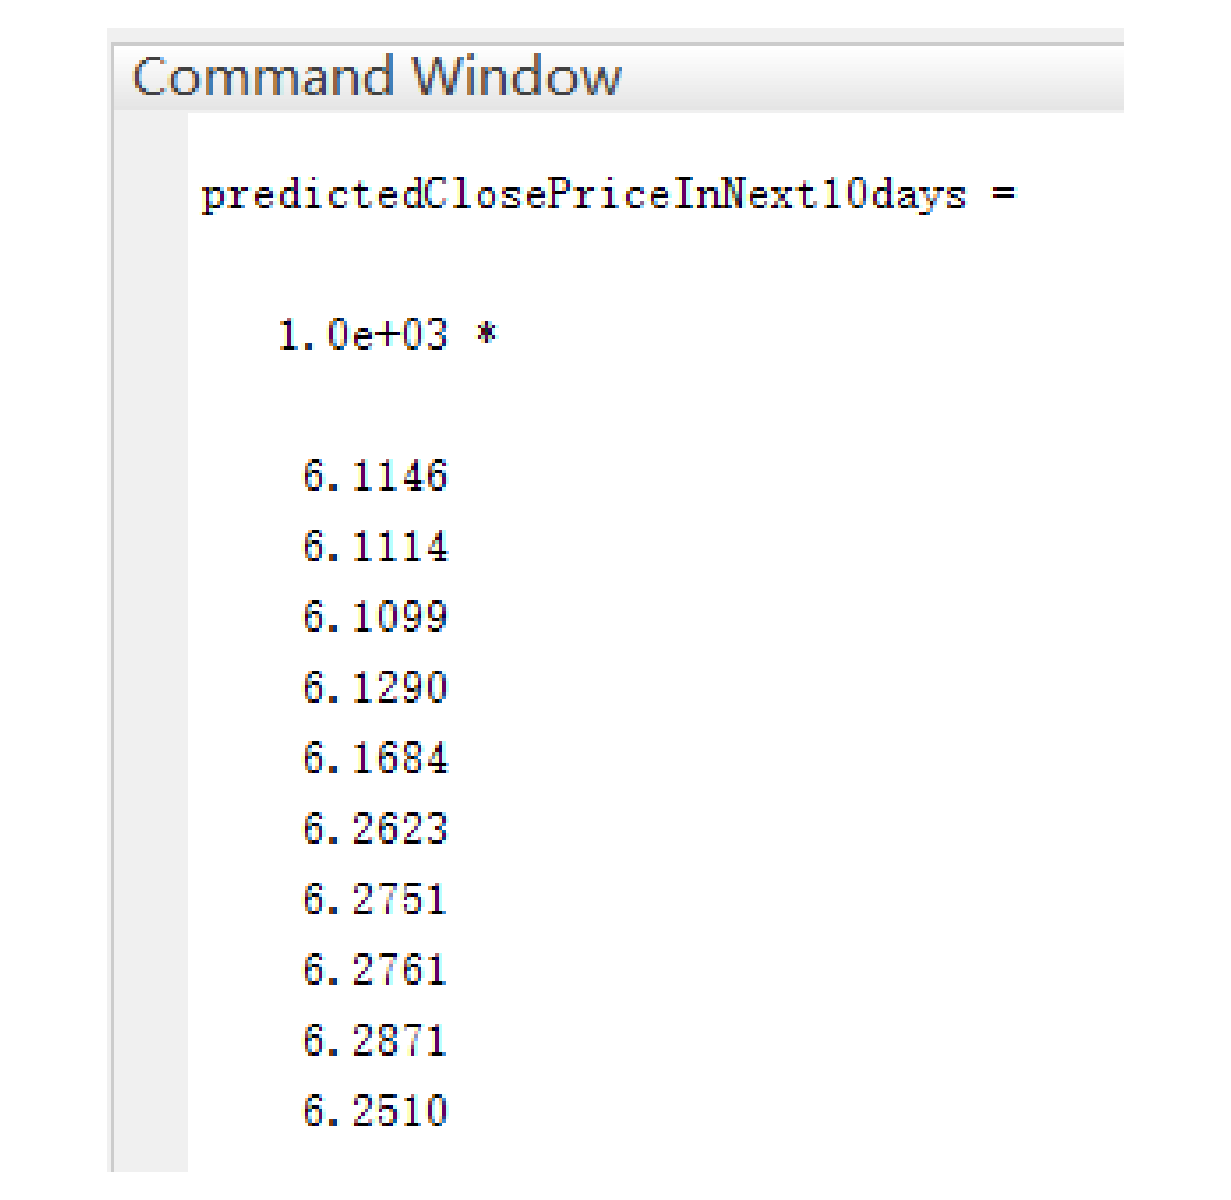
\includegraphics[width=0.45\textwidth]{image/8command.eps}}
 \caption{Free running model}
\end{figure}
\paragraph{•}As we can see, red line is the true prices and blue line is predicted prices. The accuracies of two methods are both not very accurate. But the result of multi-step ahead prediction is a little better than free running model. 
\newpage 
\paragraph{•}Next, I predicted the close prices of 10 days after 2015/12/09. The 10 true prices are unknown, so validation is not accessible.
\begin{figure}[htbp]
 \centering
 \subfigure[Next 10 days after 2015/12/09]
 {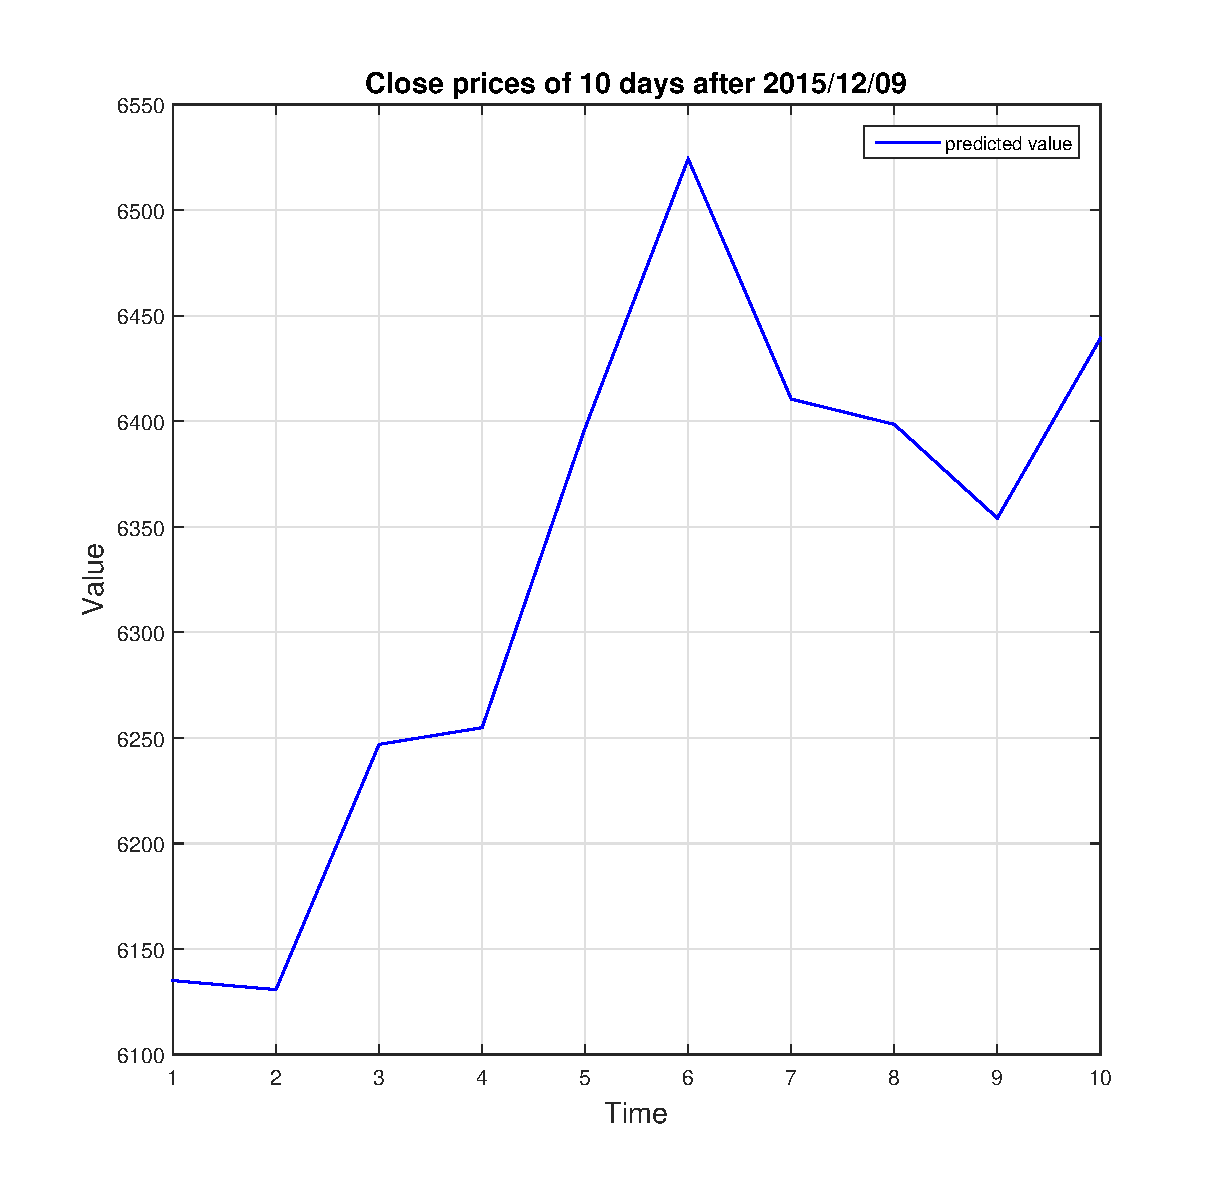
\includegraphics[width=0.45\textwidth]{image/11.eps}}
 \subfigure[Predicted output values]
 {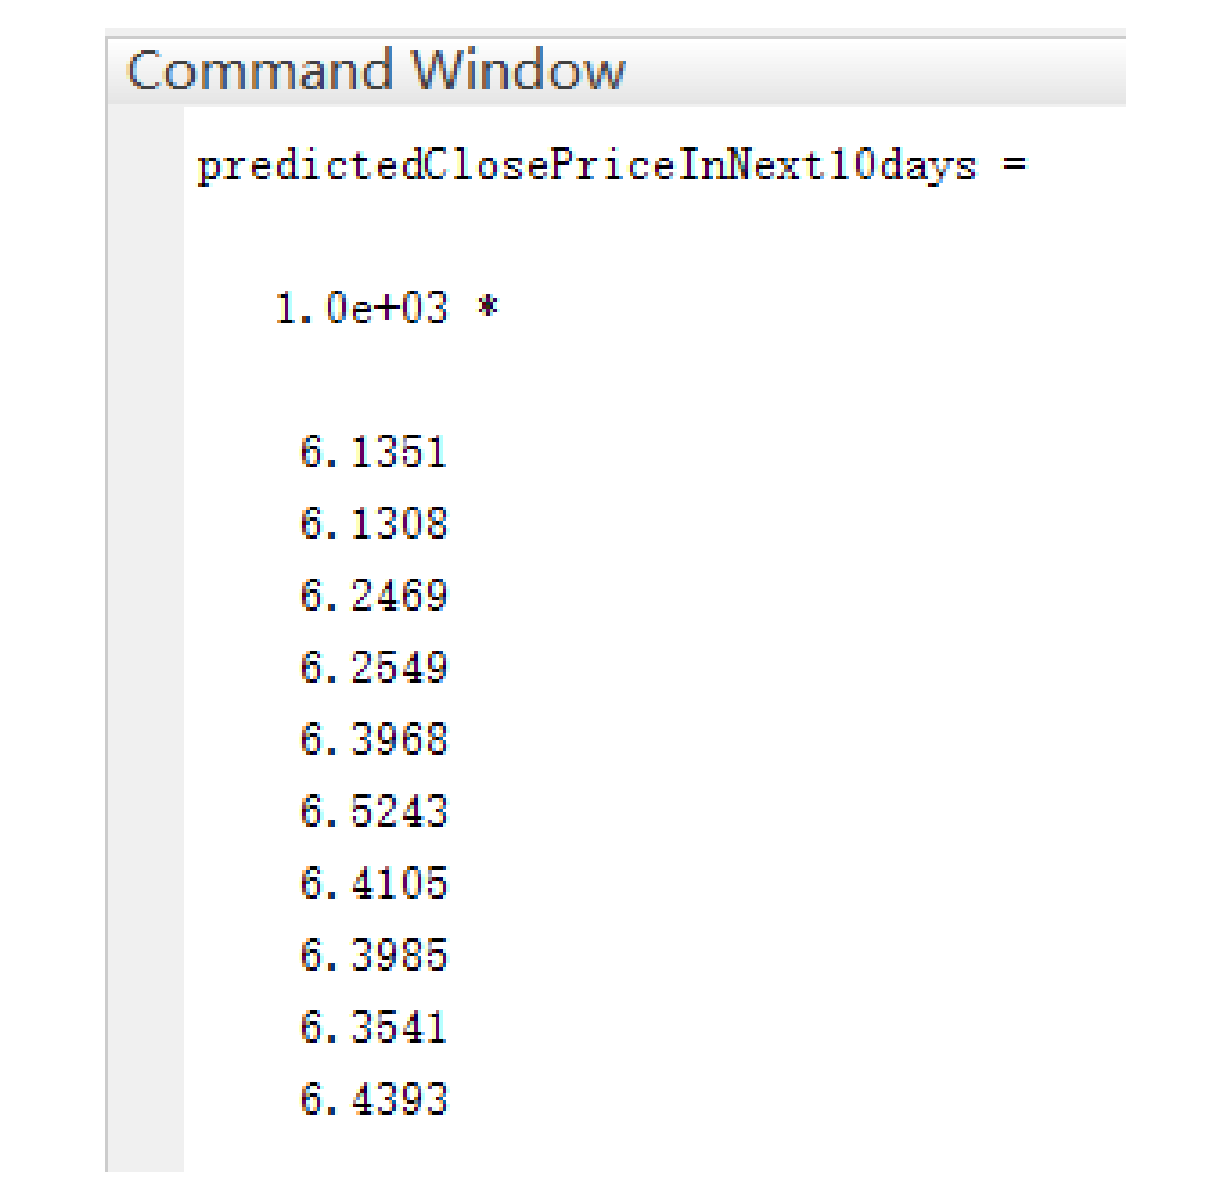
\includegraphics[width=0.45\textwidth]{image/11command.eps}}
 \caption{multi-step ahead prediction}
\end{figure}
\paragraph{Conclusion}If I am asked whether it can be used to make money, I won't make money only depending on these theory. Firstly, the time series prediction I did only depended on one factor(close price). I should consider more and more influential factors to train my model. In addition, Stock Market is fickle and can be controlled by people. This prediction method is dependent on the previous data to structure a model. It uses past to predict future. So, I think we can use this theory to estimate future stock market, which can be seen as a reference.
\end{document} 





%\(
%	\left. 
%      W=2C^{-1}(m_{2}-m_{1})=2
%    \right.
%    \left[ 
%      \begin{array}{lcr} 
%        2/3 & -1/3 \\ 
%        -1/3 & 2/3 
%      \end{array} 
%    \right]
%    \left[ 
%      \begin{array}{lcr} 
%        1.5 \\ 
%        -2 
%      \end{array} 
%    \right]
%    \left. 
%      =2
%    \right. 
%    \left[ 
%      \begin{array}{lcr} 
%        5/3 \\ 
%        -11/6 
%      \end{array} 
%    \right]  
%    \left. 
%      =
%    \right. 
%    \left[ 
%      \begin{array}{lcr} 
%        10/3 \\ 
%        -11/3 
%      \end{array} 
%    \right]    
%\)







%\section{Radial Basis Functions (RBF), Compare training and test errors}
%\begin{figure}[htbp]
% \centering
% \subfigure[Training]
% {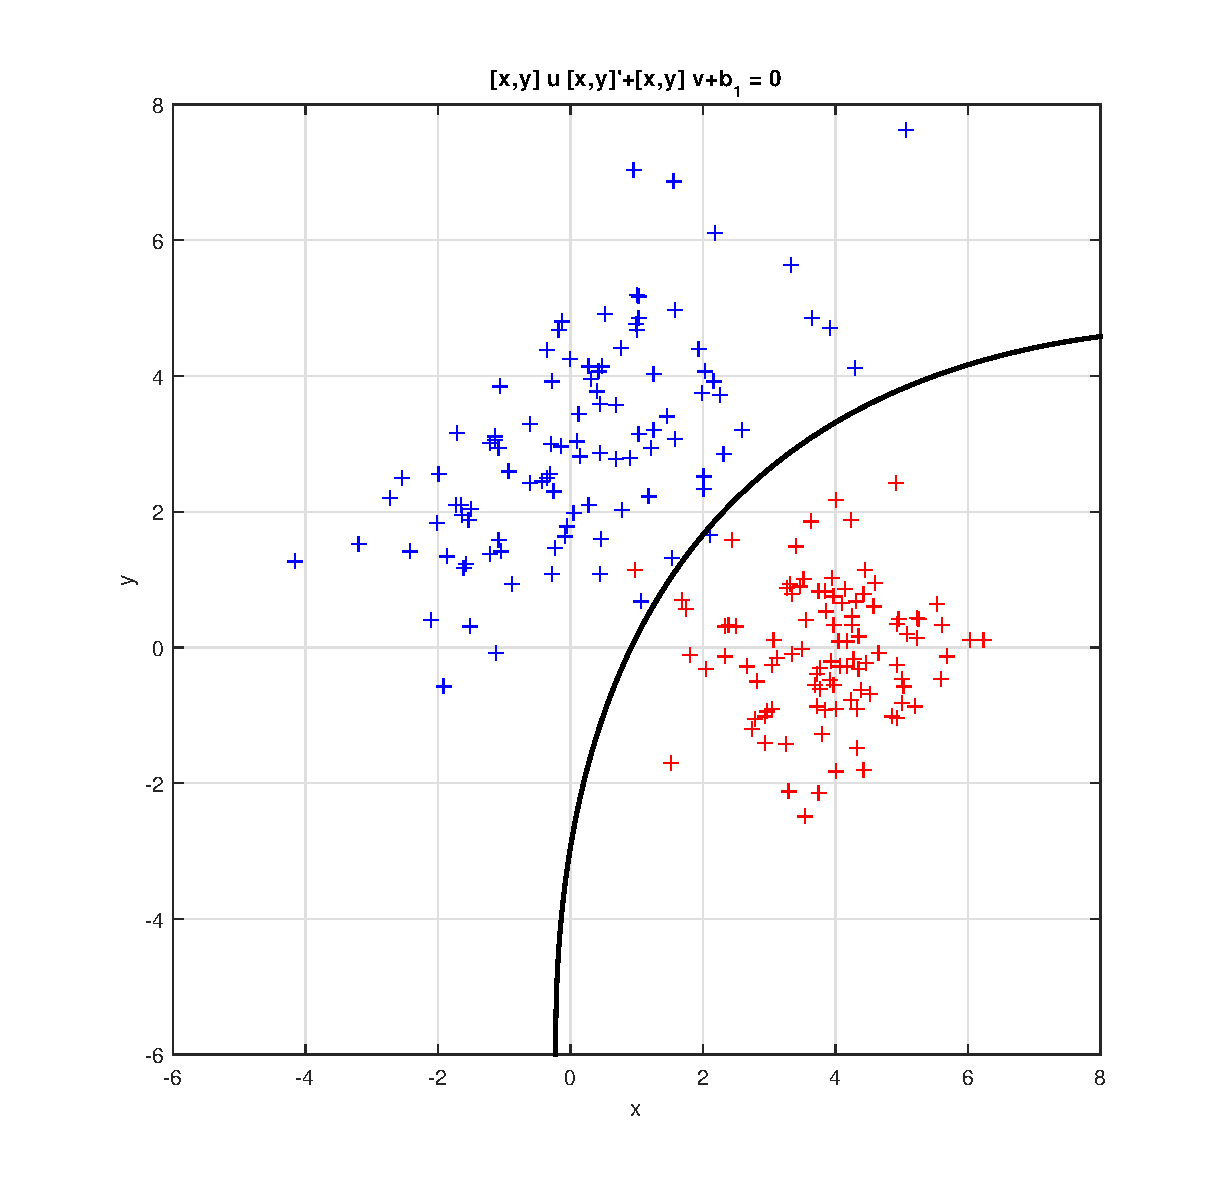
\includegraphics[width=0.39\textwidth]{image/1.eps}}
% \subfigure[Test]
% {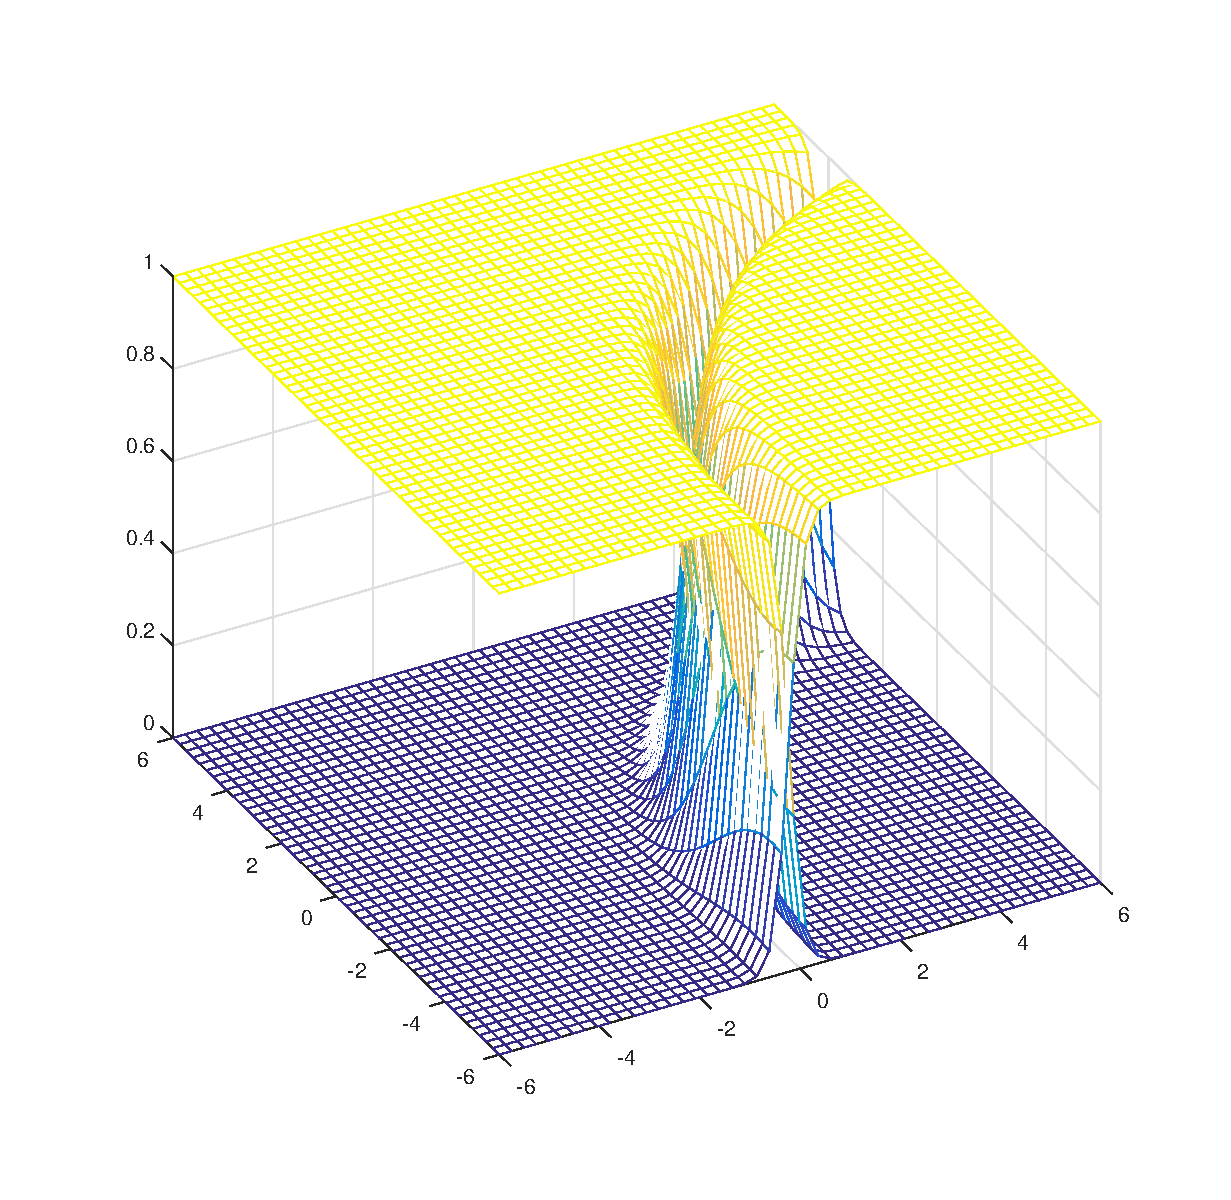
\includegraphics[width=0.39\textwidth]{image/2.eps}}
% \caption{RBF on training and test data}
%\end{figure}
%\begin{figure}[htbp]
% \centering
% \subfigure[Compare training and test errors(\textcolor{red}{K=25})]
% {\includegraphics[width=0.39\textwidth]{image1/TrTsK25.eps}}
% \subfigure[The mean of MSE of training and test data]
% {\includegraphics[width=0.39\textwidth]{image1/DK2err8.eps}}
% \caption{Compare training and test errors}
%\end{figure}
%\paragraph{•}Training errors are smaller than test errors, and training data are more centralized [Figure 2 (a)]. In addition, with the increasing of K, the error of training data is smaller and smaller to approach zero [Figure 2 (b)]. But the error of test data will be lowest in K interval \textcolor{red}{[60,100]}.
%\section{Compare with the linear regression model}
%\begin{figure}[htbp]
% \centering
% \subfigure[\textcolor{red}{K=60}]
% {\includegraphics[width=0.43\textwidth]{image1/LRK60.eps}}
% \subfigure[\textcolor{red}{K=100}]
% {\includegraphics[width=0.43\textwidth]{image1/LRK100.eps}}
% \caption{Compare linear and non-linear model}
%\end{figure}
%\paragraph{•}We can choose k=60 or 100 depending on the result of section 1, which can make the error of test data(RBF) as small as possible. We can see that non-linear model can improve predictions. 
%\section{Use different dataset on UCI: (airfoil\_self\_noise.data)}
%\begin{tabular}{|c|c|c|c|c|c|}
%\hline 
%Data Set Characteristics:  & Multivariate & Number of Instances: & 1503 & Area: & Physical \\ 
%\hline 
%Attribute Characteristics: & Real & Number of Attributes: & 6 & Date Donated & 2014-03-04 \\ 
%\hline 
%\end{tabular} 
%\begin{figure}[htbp]
% \centering
% \subfigure[\textcolor{red}{K=75}]
% {\includegraphics[width=0.41\textwidth]{image1/NoiseLRK75.eps}}
% \subfigure[\textcolor{red}{K=100}]
% {\includegraphics[width=0.41\textwidth]{image1/NoiseLRK100.eps}}
% \caption{Compare linear and non-linear model}
%\end{figure}
%\paragraph{Conclusion}RBF can solve multi-model problem better than linear regression. But the number of K is very important. We can choose a K which makes the Mean Squared Prediction Error lowest.







